% !TeX spellcheck = cs_CZ

\documentclass[a4paper]{article}
\usepackage[english]{babel}
\usepackage[utf8x]{inputenc}
\usepackage[T1]{fontenc}
\usepackage{listings}
\usepackage[a4paper,margin=2cm]{geometry}
\usepackage{amsmath}
\usepackage{graphicx}
\usepackage[colorinlistoftodos]{todonotes}
\usepackage[colorlinks=true, allcolors=blue]{hyperref}
\usepackage{wasysym} % smileys
\usepackage{fancyhdr}
\setlength\parindent{0pt} % indent

% my commands:
\newcommand{\n}{\newline}
\newcommand{\tab}{\hspace{1cm}}

\begin{document}

\title{Ptakopět \\ \large Překlad tam a kntrolně zpět }
\author{Vilém Zouhar}
\date{November to December 2018 \\ Rev. 2}
\maketitle 

% https://www.cs.uic.edu/~jbell/CourseNotes/OO_SoftwareEngineering/SE_Project_Report_Template.pdf

\section*{Overview}
Ptakopět (Překlad Tam A KOntrolně zPĚT) is an agile browser agnostic plugin, which aims to help people translate to languages, where they are unable to verify the quality of the translation, by offering backward translation of the result.

\subsection*{The purpose of the project}
The issue at hand is known as \textit{Outbound Translation}. Many users use machine translation to verify their own translation, or can at least affirm, that the machine translation is valid. Translation systems are, however, not perfect and despite their great power, they tend to perform poorly on unprecedenced phenomena (unknown words, unexpected word order, etc.). Users translating to languages, which they don't master enough to validate the translation could use Ptakopět to verify (and assure them), that the machine translation output is valid. As many encounters with foreign languages happen on the Internet, Ptakopět is developed as a browser extension.

\subsection*{Other solutions}
Backwards translation is only one of the solutions to \textit{Outbound Translation}. Other could inlude more autonomous systems, such as text highlighting or numeric responses. Backward translation relies on the ability of the user to asses the differences between texts.

\subsection*{The scope}
Ptakopět aims to provide a backward translation interface to already existing translation engines. It does not do the translation itself in any way. Existing translation backends are provided by the Charles University, namely by Martin Popel and other associates. The interface is provided in a form of browser agnostic plugin, that can also be hardwired to website as a plain script.

\vspace{1cm}
\begin{center}
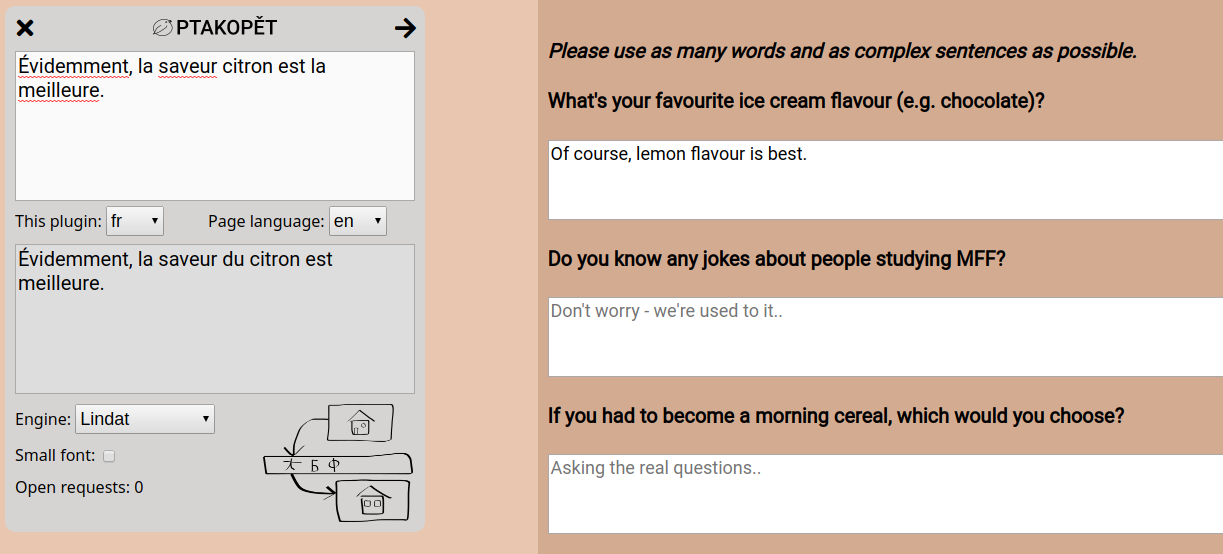
\includegraphics[width=\textwidth]{screenshot_3}
\end{center}

\section*{Implementation}
The plugin itself is written in JavaScript, but injects HTML, CSS and jQuery framework into webpage. Making the plugin indifferent to whether it is run as a background sciprt (browser plugin) or as an user script (included in webpage) posed a substantial obstacle. Resulting implementation works, but is unfortunately affected by web styling. Eg.  website CSS can define the looks of the plugin, which is not intended and can result in usable, but not aesthetically pleasing design. \\
Ptakopět tries to capture all input events to \textit{textareas} and \textit{inputs}. This is a very robust approach, but about half of the websites (as of 2018) use custom input elements (to provide styling and extra functionaliy). As a result, these elements can't be captured using Ptakopět. This is obviously a radical usability issue, but we didn't find any universal solution to this problem. \\
Text events are processed and forwarded to translation engine using AJAX requests. This could eventually pose a threat to these backends, if the plugin was used by many people simultaniously. The engines would be glutted by requests, as every keypress invokes one or two translations. They are indistinguishable from legit requests, as the plugin works user-side. This could be solved by postponing requests to some interval of no key press (standard approach).

\subsection*{Technical details}
The code itself is located in the \textit{src/} directory. The \textit{manifest.json} file is obligatory for all plugin versions. When Ptakopět is run as a background script (browser plugin), then \textit{ptakopte\_background\_bootstrap.js} is executed, which adds listeners to context menu and icons. Then \textit{ptakopet\_init.js} is run as a user script and from this point on, it is identical to having the script run from the webpage. Due to asynchronous loading, the startup functions are called in \textit{ptakopte\_init\_user.js}. Generally, \textit{ptakopet\_init.js} handles visual elements (eg. displaying \textit{floater.html}, CSS etc.), while \textit{ptakopet\_translator.js} takes care of the translation flow. Ptakopět was designed to support fast addition of new translator backends or supported languages. Each translation object in Ptakopět manages it's own AJAX requests in standardized form.

\vspace{1cm}
\begin{center}
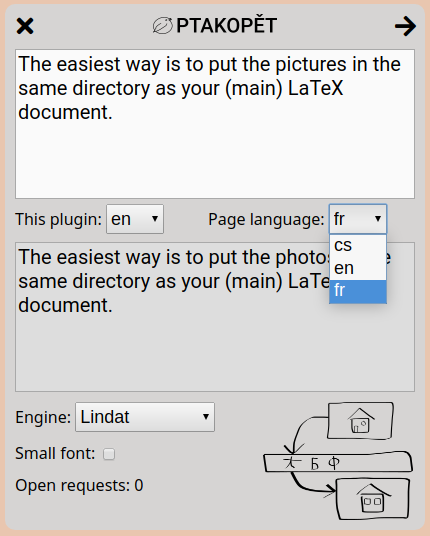
\includegraphics[width=0.35\textwidth]{screenshot_4}
\end{center}
\begin{center}
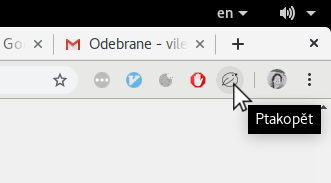
\includegraphics[width=0.4\textwidth]{screenshot_5}
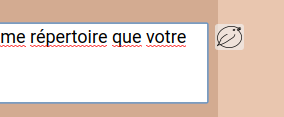
\includegraphics[width=0.4\textwidth]{screenshot_6}
\end{center}

\section*{Publishing}
Ptakopět was published online. Basic demonstration and info is located at \href{http://ptakopet.vilda.net}{ptakopet.vilda.net}. Ptakopět was also presented at MFF Open Days, but for technical reasons we were unable to collect data. The presentation page is locate at \href{https://vilda.net/s/dod\_ptakopet}{vilda.net/s/dod\_ptakopet}. The plugin itself is distributed as a \href{https://chrome.google.com/webstore/detail/ptakop\%C4\%9Bt/hgjlgmhmcmcmjiclegnipnaeejpibjmn}{Chrome} and \href{https://addons.mozilla.org/en-US/firefox/addon/ptakop\%C4\%9Bt/}{Firefox} extension. The plugin was also submitted to the Opera addon store, but still hasn't been reviewed.
Source code is published at a GitHub repository: \href{https://github.com/zouharvi/ptakopet}{github.com/zouharvi/ptakopet}, the licence not yet decided, but feedback and code contributions welcome.

\section*{Possible extensions}
Future versions could also include a full fledged web interface similar to that of Google Translate (one page). Since Ptakopět is somewhat limited to backend capabilities, their extension is also desired.

\section*{Conclusion}
The first version of Ptakopět met all imposed usability criteria and didn't exceed expected amount of work required. 

\end{document}
